\section{Mechanical Design}

The mechanical project of the robot was completely redefined. New devices such as the chip kick and the improvement of the transmission system were developed. This totally new robot was designed and built using CAD (Computer Aided Design) and CAM (Computer Aided Manufacturing) software, moreover extensive testing was done to reach the current project.

\begin{figure}[thpb]
	\centering
	\subfigure[]{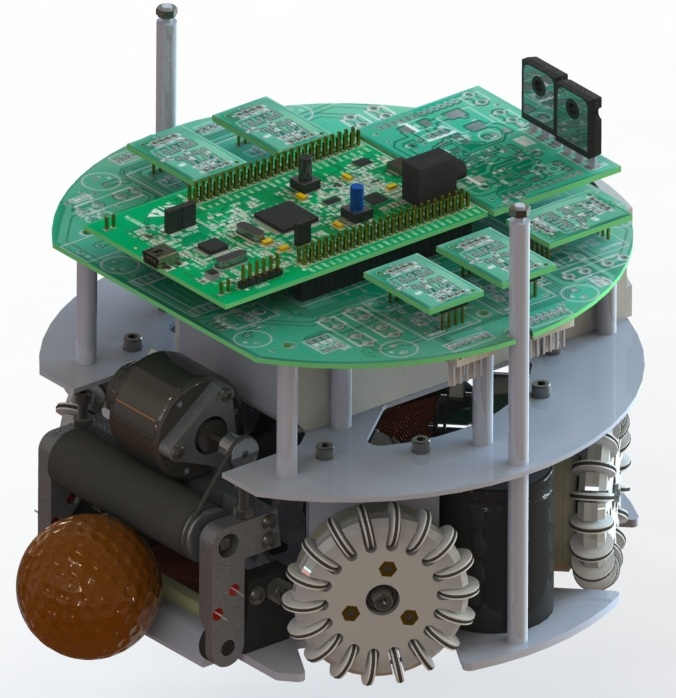
\includegraphics[width = 0.425 \textwidth]{img/cad.jpg}}
	\subfigure[]{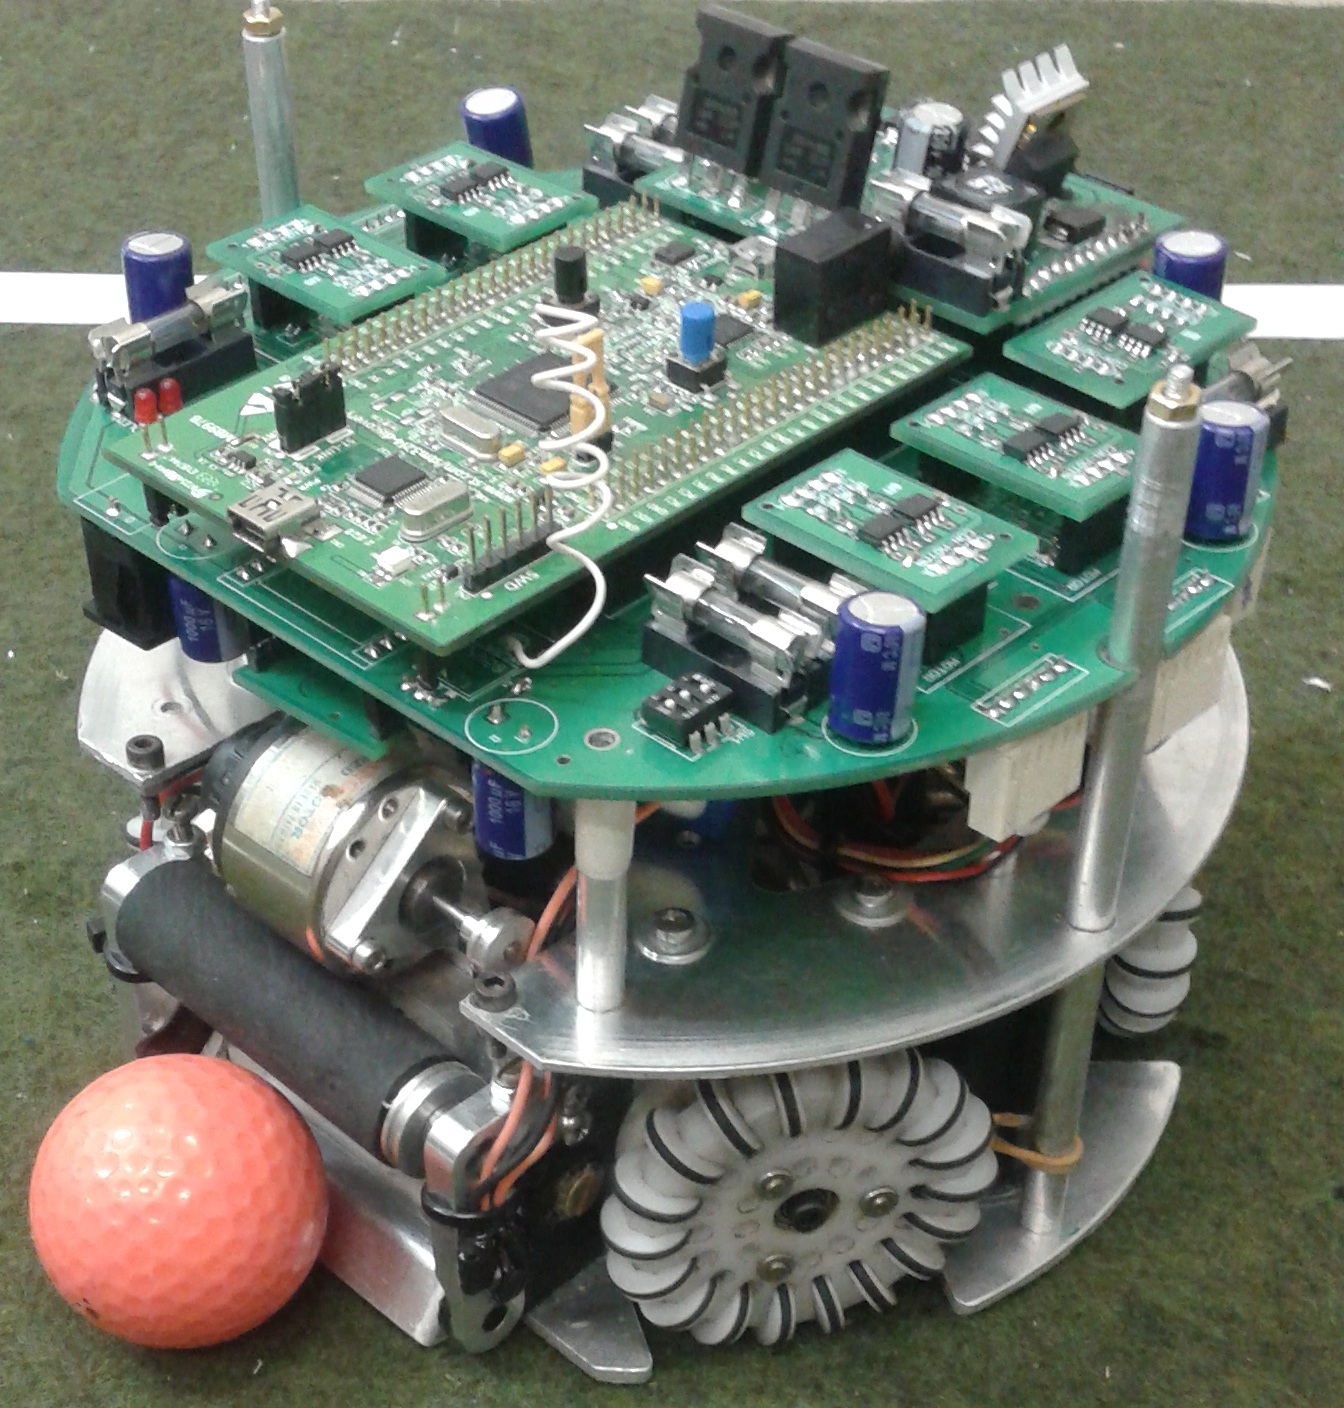
\includegraphics[width = 0.4 \textwidth]{img/real.jpg}}
	\caption{(a) Mechanical 3D model view. (b) Robot view.}
	\label{mec}
\end{figure}

Figure \ref{mec} shows mechanical
3D view and real view of the robot.

\subsection{Dimensional Constraints}

In compliance with the SSL rules, the height of the robot is 149 mm and the maximum projection of the robot on the ground is 180 mm.

With the CAD software we were able to measure the percentage of the ball area that was covered by the robot. The maximum percentage of ball coverage found was 19,8 \%, according to the 20/80 rule of the league. 

\begin{figure}[thpb]
	\centering
	\subfigure[]{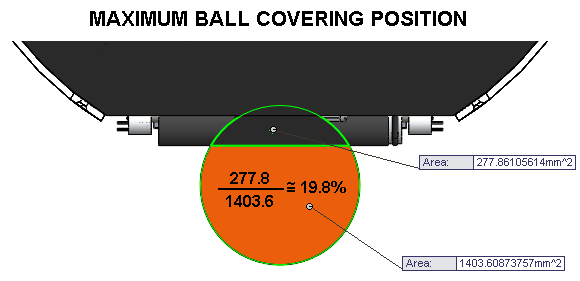
\includegraphics[width = 0.425 \textwidth]{img/20-80_rule.png}}
	\caption[]{Maximum covered area of the ball}
	\label{mec}
\end{figure}

\subsection{Transmission System}

A system of internal gears was made to transmit the power of the engines to the wheels. This system has several advantages compared to traditional gear meshing. Avoiding debris entering the engine, creating a cavity to apply grease for lubrication of gears and an overall size are some of them.

However there are some difficulties in the manufacture of this part, mainly due to the small size of the teeth needed to mesh with standard engine gear (the distance between to consecutive teeth is less than 1 mm). Thus it was not feasible to machine the internal gear, so it was decided for the 3D printing process in ABS plastic.

Some prototyping have been done ensure accuracy and strength of the gear. In previously models the gears were made out of aluminium, much harder than the ABS plastic. For best results we pursued for a high accuracy 3D printing process. In this way we were able to get a better shape from the teeth: avoiding cracks in the structure and achieving a solid and precise part.

\begin{figure}[thpb]
	\centering
	\subfigure[]{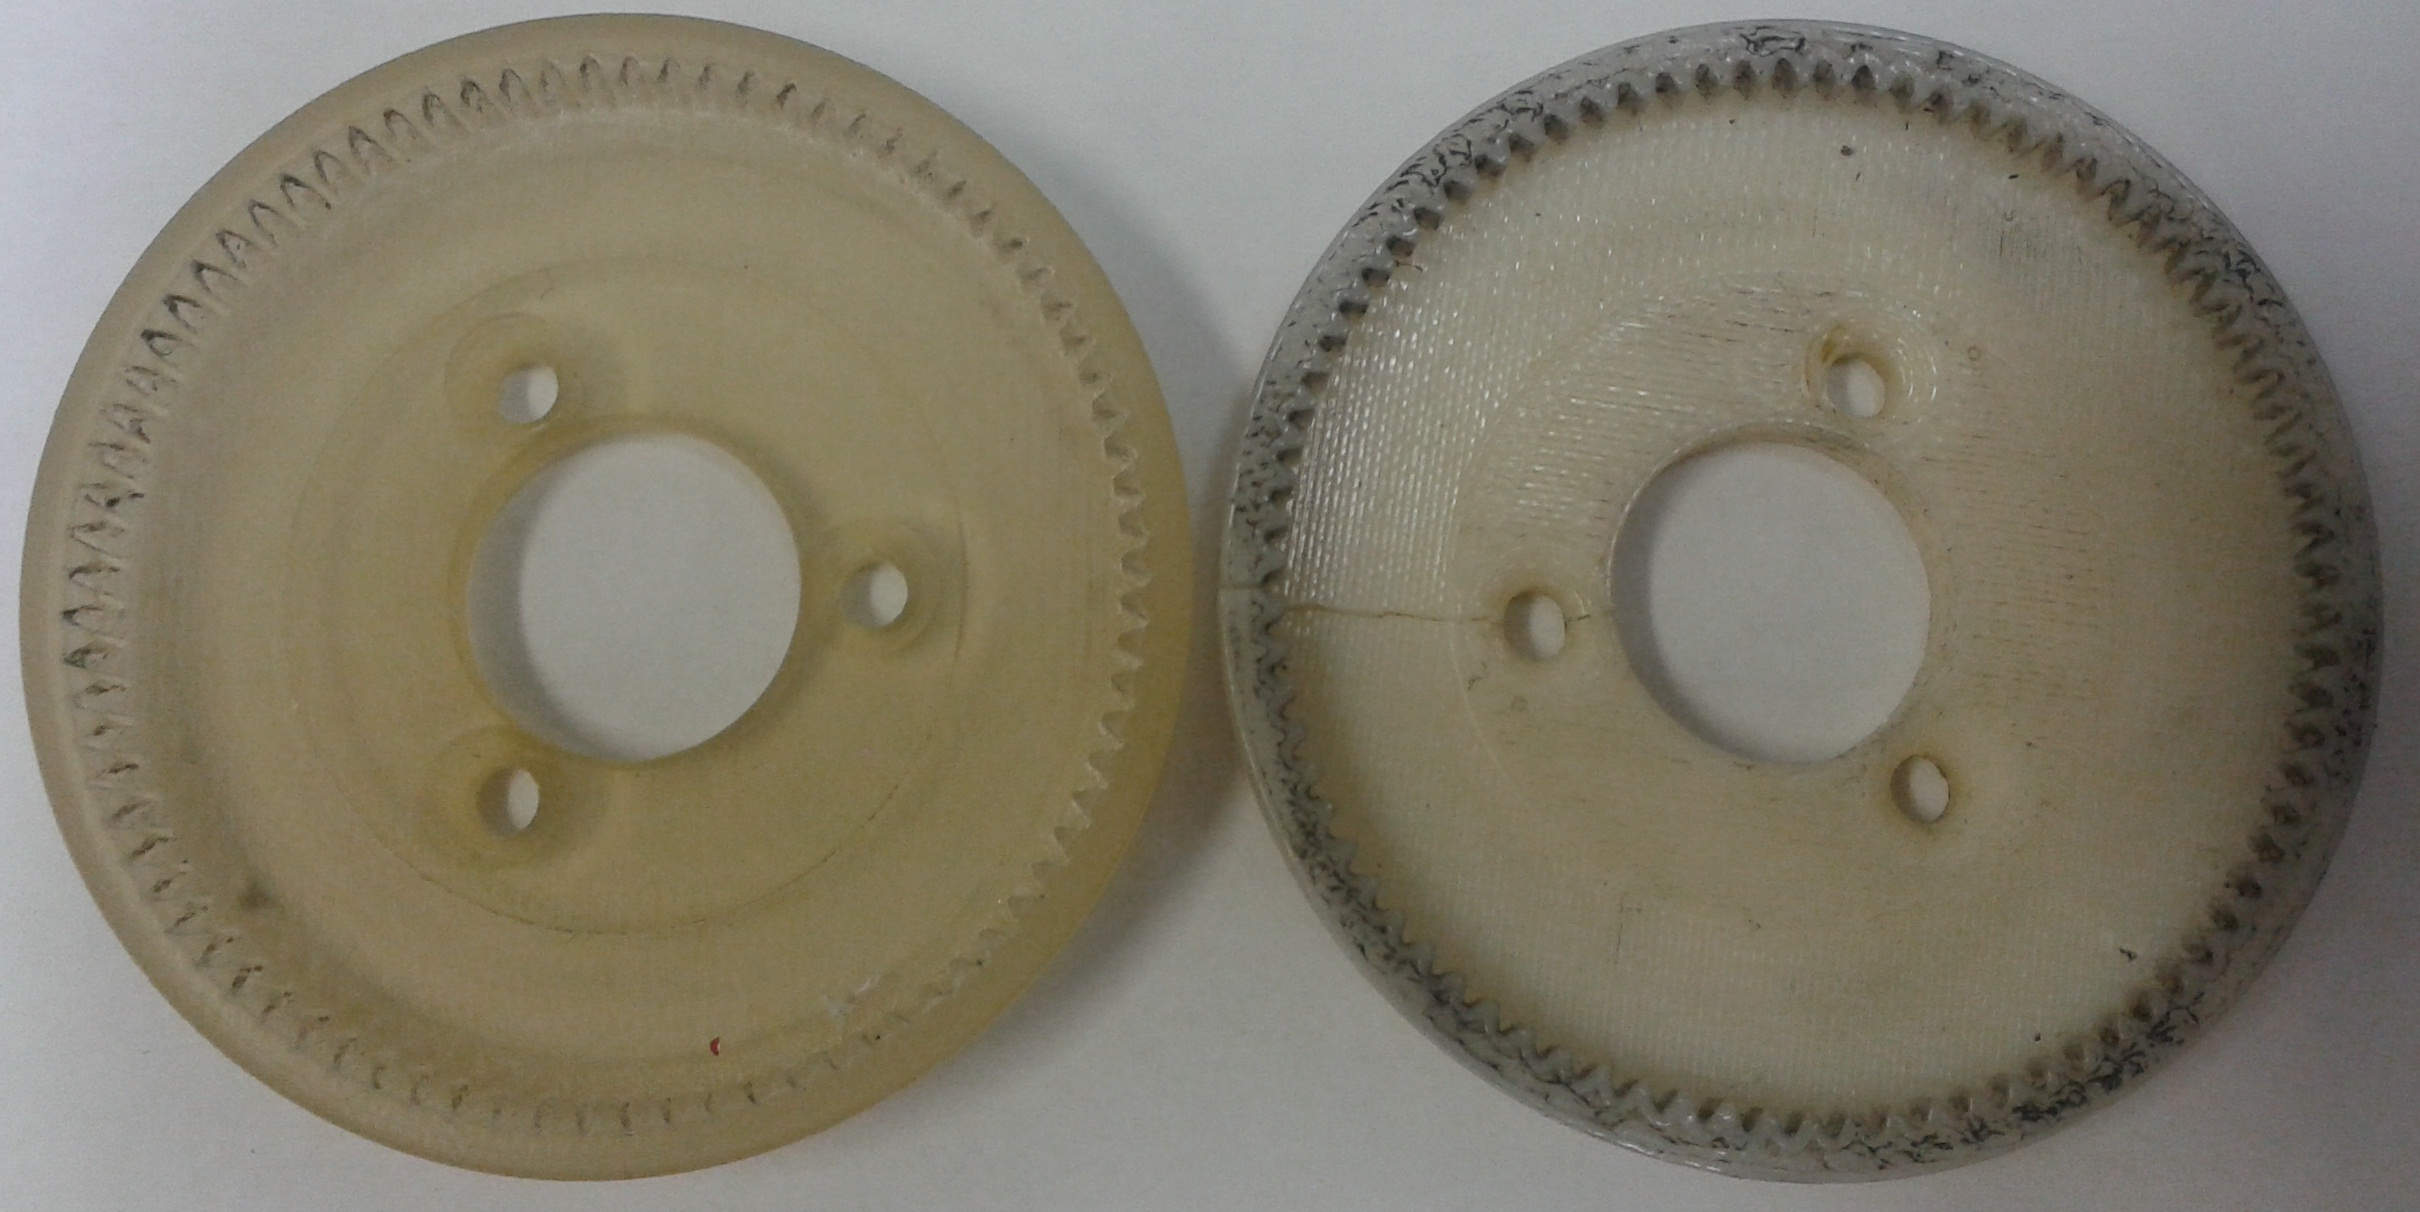
\includegraphics[width = 0.425 \textwidth]{img/gears.jpg}}
	\caption{(a) High precision 3D printed internal gear. (b) Cracked gear (lower precision).}
	\label{mec}
\end{figure}

Full power stoppage tests were performed, locking the motor, bringing the gear to its limit. Satisfactory result were achieved making the system very reliable.

\subsection{Chip Kick}

The chip kick is based on a flat solenoid, which is mounted in a slot at the chassis (close to the ground). When activated the core of mild steel is accelerated against the rear of the chip, which revolves around it's axis and makes the ball rise. Due to the limited space, complex construction and details, we also chosen the 3D printing as the manufacturing process.

\begin{figure}[thpb]
	\centering
	\subfigure[]{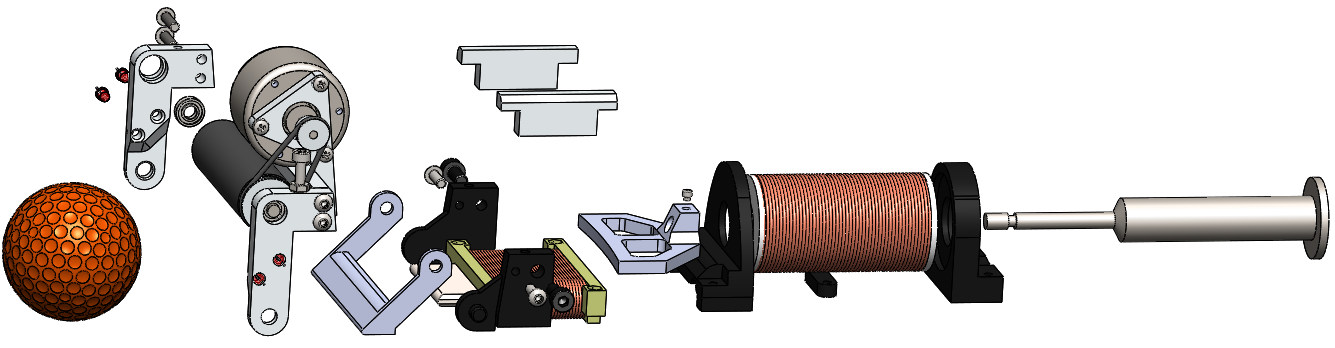
\includegraphics[width = 0.425 \textwidth]{img/sistema2.png}}
	\subfigure[]{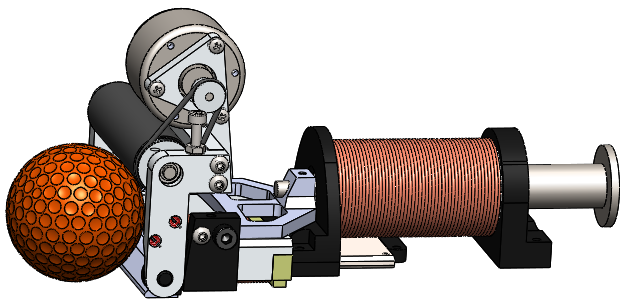
\includegraphics[width = 0.4 \textwidth]{img/sistema3.png}}
	\caption{(a) Dribbler, chipper and kicker assembly. (b) Exploded view.}
	\label{mec}
\end{figure}

The flat solenoid is assembled in a way that work as a guide rail for the kick plunger as well. We are using rubber-bands to pull back the chipper and the kicker plungers to keep the simplicity of the mechanism.
